\documentclass[11pt]{article} 

%\usepackage{fontspec}
%\setmainfont{Arial}
\usepackage{amsmath,amsfonts,amssymb,pxfonts,xspace}
\usepackage{graphicx, ragged2e}
\usepackage{pgffor}
%\usepackage{ulem}
\usepackage{caption}
\usepackage{courier}

\usepackage{verbatim}
%\usepackage[usenames,dvipsnames]{xcolor}                                 
\usepackage{listings}

\usepackage{float}
\usepackage{subfig}

%\graphicspath{{./figures/}}                                          
\newcommand{\bllt}{\item \small}
\newcommand{\doneTaskNoItem}[1]{\sout{#1}}
\newcommand{\doneTask}[1]{\item \sout{#1}}
\newcommand{\doneTaskHyp}[1]{\item \textcolor{blue} {\sout{#1}}}
\newcommand{\optTask}[1]{\item  \textcolor{green}{#1}}
\newcommand{\prioTask}[1]{\item  \textcolor{red}{#1}}
\newcommand{\timeEst}[1]{\textit{Time:} \textit{#1}}
\newcommand{\te}[1]{\textit{TimeEst:} \textit{#1}}
\newcommand{\priority}[1]{\textit{Priority:} \textit{#1}}
\newcommand{\pr}[1]{\textit{Priority:} \textit{#1}}
\newcommand{\prio}[1]{\textit{Priority:} \textit{#1}}
\newcommand{\dueBy}[1]{\textit{Deadline:} \textit{#1}}
\newcommand{\MyName}{Vivek~Kale}
\newcommand{\fixme}[1]{\textcolor{blue}{[FIXME: #1]}}
\newcommand{\revision}[1]{\textcolor{blue}{[FIXME comment : #1]}}
\newcommand{\regItem}[1]{\item \textcolor{cyan}{#1}}
\newcommand{\regRoutineItem}[1]{\item \textcolor{green}{\textit{Reg. Routine:} #1}}
\newcommand{\situationItem}[1]{\item \textcolor{magenta}{\textit{Situation:} #1}}
\newcommand{\deadline}[1]{#1}
\newcommand{\dl}[1]{\textit{Deadline:}#1}

\newcommand{\comments}[1]{} 

%TODO: figure out better title for this file 
%TODO: add in all relevant packages 
%TODO: do a clean-up for writing/how-to-say-it and visual appeal 
%TODO: add in more on summary page  
%TODO: add in all howtos 
%TODO: try to get multi-column for month plan doc. 


\usepackage[normalem]{ulem}

\usepackage{amssymb}
\usepackage{amsmath}
\usepackage{caption}
\usepackage{courier}
\usepackage[usenames,dvipsnames]{xcolor}
\usepackage{listings}
\usepackage{float}
\usepackage{subfig}
\usepackage{tikz}

\usetikzlibrary{decorations.pathreplacing,calc}
\newcommand{\tikzmark}[1]{\tikz[overlay,remember picture] \node (#1)
  {};}

\newcommand*{\AddLstNote}[4]{%                                                                                       
    \begin{tikzpicture}[overlay, remember picture]
        \draw [decoration={brace,amplitude=0.5em},decorate,ultra
          thick,red]
            ($(#3)!([yshift=1.5ex]#1)!($(#3)-(0,1)$)$) --
            ($(#3)!(#2)!($(#3)-(0,1)$)$)
                node [align=center, text width=2.5cm, pos=0.5,
                  anchor=west] {#4};
    \end{tikzpicture}
}%                                                                   

\makeatletter
% \bibalias{<alias>}{<source>} makes \cite{<alias>} equivalent to
% \cite{<source>}                                   
\newcommand\bibalias[2]{%                                   
  \@namedef{bibali@#1}{#2}%                                          
}

\lstset{
        language=C++,
        basicstyle=\tiny\ttfamily, % Standardschrift                          
                                    % % TODO: consider making tiny to
                                    % % make                         
                                     % % things fit                        
         numbers=none,               % Ort der Zeilennummern                                                         
         numberstyle=\footnotesize\ttfamily,          % Stil der
                                % Zeilennummern                                       
         %stepnumber=2,               % Abstand zwischen den
         %Zeilennummern                                           
         numbersep=6pt,              % Abstand der Nummern zum Text                                                  
         tabsize=2,                  % Groesse von Tabs                                                              
         extendedchars=true,         %                                                                               
        breaklines=true,            % Zeilen werden Umgebrochen                                                      
        frame=single,
         keywordstyle=[1]\textbf,    % Stil der Keywords                                                             
         stringstyle=\ttfamily,
         showspaces=false,           % Leerzeichen anzeigen ?                                                        
         showtabs=false,             % Tabs anzeigen ?                                                               
%         xleftmargin=17pt,                                                                                          
%         framexleftmargin=17pt,                                                                                     
%        framexrightmargin=5pt,                                                                                      
%         framexbottommargin=4pt,                                                                                             backgroundcolor=\color{white!97!black},
         showstringspaces=false      % Leerzeichen in Strings anzeigen
                                % ?                                             
}

\title{} 
\author{}

%REMINDER: uncomment the below later. 
\title{CS598WG Final Project}
\author{Vivek Kale}

\begin{document}
\maketitle

%\textbf{Summary:} This document contains the homework 4 for CS598WG
%Spring 2015. 
%\newpage 

%TODO: could update the below to be more clear.  
\section{Introduction} 
In this report, I consider the utility of within-node load balancing for
MPI+OpenMP codes that suffer from application-level load imbalance (as
opposed to codes that suffer from load imbalances independent of the
application, e.g., a load imbalance induced by OS daemons). 

In prior work of mine, I worked on within-node load balancing
strategies specifically developed to mitigate load imbalance caused
by operating system interference. These same strategies were then
applied to some applications suffering from application-level
imbalance, with some optimizations to the load balancing strategy done
to improve performance of these applications. 

This project aimed at detailed characterization of load imbalance in
one particular code. The particular code is the Lonestar Barnes-Hut
benchmark~\cite{LonestarBH} from University of Texas at Austin. It
calculates movement of particles under influence of gravity over a
series of timesteps. 

The first question we ask is whether significant load imbalance exists
across different cores. This imbalance will be quantified. The
conjecture we explore is that the load distribution across thread
is persistent over simulation timesteps on a multi-core node. 
This will be analyzed with a detailed analysis through correlation of
thread load across consecutive timesteps. To understand the cause of
persistence, we make and explore another conjecture that
individual particle loads themselves tend to persist over
timesteps. This requires a more detailed correlation analysis, which
is described later. 

%I display the load imbalance across cores through showing the timings
%across threads for each timestep. I then show persistence of load
%imbalance through correlation metrics. 

\section{Performance Expectation}
Barnes-Hut is a code where particles are organized in an oct-tree data
structure. Typically, particles vary non-uniformly over the
space~\cite{BarnesHutPaper}. In some regions, particle density may be
very high while other regions may be almost empty. The oct-tree is
used to approximate forces due to far-away particles. As a result, the
first performance expectation is that the load on different particles
will be substantially different. Secondly, this particle load
variation will lead to loads being substantially different across
threads, even though each thread may have a mixture of high load and
low load particles. 

Since particles likely move slowly in molecular dynamics simulations,
i.e., in each simulation timestep they move to nearby
locations~\cite{SpaceFilling}, one can expect that the load variation
persists from one timestep to the next. The load distribution across
particles, as well as threads, will be similar from 
one timestep to the next, even though it may change substantially over
a large number of timesteps. A corrollary of the above is an
expectation that if the ratio of maximum load to average load across all threads in timestep i is, say,
1.5, then the ratio in the next timestep will be close to 1.5.

%On average, this would be 1.5 times the total load divided by the
%number of cores. Also, on each timestep, the performance could be
%improved. 
%The same imbalance would occur on each timestep. Thus, we
%can multiply this extended time per timestep for a single, arbitrary
%node, by the number of timesteps. 

\section{Experiments}
We ran on two different problem sizes of the Barnes-Hut 
code~\cite{LonestarBH}, one with 10,000 particles and one with 100,000
particles. The first problem ran for 50 timesteps, and the second for 
75 timesteps. We ran the code on a node of the taub cluster, a 12-core
NUMA architecture. We modified the Barnes-Hut code to measure the
timestep timings, as shown in Figure~\ref{code:timestepTimings}. 

\begin{figure}[ht!]
\label{code:timestepTimings}
\begin{lstlisting}
gettimeofday(&starttime, NULL);
 for (int i = start; i < end; i++) {
    body[i]->ComputeForce(groot, gdiameter);
  }
gettimeofday(&endtime, NULL);
runtime = (long) (endtime.tv_sec * 1000.0 + endtime.tv_usec / 1000.0 -
starttime.tv_sec * 1000.0 - starttime.tv_usec / 1000.0 + 0.5);
timings[slice][step] = runtime;
\end{lstlisting}
\caption{\label{code:timestepTimings} Barnes-Hut code modification for
  timing of each simulation timestep, for each thread.} 
\end{figure}

\begin{figure}[ht!]
\label{fig:timestepTimings-runB}
\begin{center}
\includegraphics[width=\textwidth]{timestepTimings-runB}
\end{center}
\caption{\label{fig:timestepTimings-runB} Load Distribution Correlation across timesteps for run with 10,000 particles.}
\end{figure}

\begin{figure}[ht!]
\label{fig:timestepTimings-runC}
\begin{center}
\includegraphics[width=\textwidth]{timestepTimings-runC}
\end{center}
\caption{\label{fig:timestepTimings-runC}Load Distribution Correlation
  across timesteps for run with 100,000 particles.}
\end{figure}

Figure~\ref{fig:timestepTimings-runB} shows the timestep timings for
different threads for the case of 10,000 particles. Here, we see that
the simulation timestep timings for each thread stays constant through
the execution of the run. Additionally, the fluctuations of timestep
timings are periodic over simulation timesteps of the
run. These results show that there exists load imbalance across cores
during execution of the code, but the results do not show any
indication of persistence of load imbalance over timesteps.
%Prior work does not show ... 
Running a Barnes-Hut (or any N-body) code on a possibly noisy multi-core
node, how much can persistence of load imbalance can we expect, in order to take advantage of it for a within-node load balancing technique?

%The above observations does not tell us whether 
To assess persistence of load distribution across threads over the
simulation timesteps, we need to determine the degree to
which the distribution of the load distribution stays
the same from one timestep to the immediately succeeding one. To
determine this degree, we use a metric which calculates a correlation
coefficient between timestep i and i+1, called Pearson's
correlation metric~\cite{PearsonsCorrel}. We use Pearson's correlation
metric because we used MS Excel to plot the data, and the formula is
used in MS Excel's CORREL function. The formula for calculating the
correlation coefficient is shown below.

%\textbf{Correlation:}\\
$$r = r_{xy} =\frac{\sum ^n _{i=1}(x_i - \bar{x})(y_i
  -\bar{y})}{\sqrt{\sum ^n _{i=1}(x_i - \bar{x})^2}
  \sqrt{\sum^n_{i=1}(y_i - \bar{y})^2}}$$ 

We apply the above equation within the context of the simulation timestep
timings results. To get the correlation coefficent for the simulation
timestep $i+1$, we plug the vector of per-thread timings on
timestep i into $x$ in the above expression, and plug the vector of
per-thread timings on timestep $i+1$ into $y$ in the above expression,
and evaluate the above expression. 

\begin{figure}[ht!]
\label{fig:timestepCorrel-runB}
\begin{center}
\includegraphics[width=0.9\textwidth]{LoadTimestepCorrel-runB}
\end{center}
\caption{\label{fig:timestepCorrel-runB}Load Distribution Correlation across timesteps for run with 10,000 particles.}
\end{figure}

\begin{figure}[ht!]
\label{fig:timestepCorrel-runC}
\begin{center}
\includegraphics[width=0.9\textwidth]{LoadTimestepsCorrel-runC}
\end{center}
\caption{\label{fig:timestepCorrel-runC}Load distribution correlation
  across timesteps for run with 100,000 particles.}
\end{figure}

Figure~\ref{fig:timestepCorrel-runB} shows the results for the
Pearson's correlation metric applied to load distribution across
threads over the timesteps for the run of 10,000 particles, and
Figure~\ref{fig:timestepCorrel-runB} for the run of 100,000
particles. For both the run of 10,000 particles and 100,000 particles,
the correlation is above 50\% between each of the simulation
timesteps. The correlation is lower for the run of 100,000 particles than for
the run of 10,000 particles. The reason for the lower correlation for
the 100,000 particle run is likely due to OS noise, since the
likelihood of occurrence of OS noise events is larger because of the
longer run: the run for 100,000 particles takes 152 seconds, while the
run for 10,000 particles takes only 26 seconds (averaged over 5
trials). 

%The cause of persistence may be due to the force calculations of the
%particles
%TODO: consider adding ``and Not due to persistence of other things
%like OS noise ..  `
% TODO: check due to

To ascertain that the cause of the persistence of imbalance is due to
persistence of individual particle loads (and not due to other effects, e.g.,
OS noise that happens to be periodic and coarse-grained), we examined
the persistence of particle timings. Since timing each particle's
force evaluation individually will be overhead-prone and generate too
large a data, we tracked the performance of particles in chunks of 100
consecutive particles. We did so by modifying the loop body of the N-body
computation, as shown in Figure~\ref{code:particleTimings}.

%imperfect partitioning across threads, and not the grouping of particles 
%themselves, we looked at the persistence of particle timings. 

\begin{figure}[ht!]
\label{code:particleTimings}
\begin{lstlisting}
for(timestep = 0; step < n; step++)
{
// ...
  start = slice * nbodies / threads;
  end = (slice + 1) * nbodies / threads;
  gettimeofday(&starttime, NULL);
  long t;
  long last =(long)(starttime.tv_sec * 1000000.0 + starttime.tv_usec);
  for (int i = start; i < end; i++) { // the iterations are independent: they can be executed in any order and in parallel
    body[i]->ComputeForce(groot, gdiameter); // compute the acceleration of each body (consumes most of the runtime)             
    if((i%100) == 99)
      {
        gettimeofday(&endtime, NULL); // get time for particle
        t = (long) (endtime.tv_sec * 1000000.0 + endtime.tv_usec);
        particleTimings2[i/100][step] = t - last;
        last = t;
      }
  }
//...
}
\end{lstlisting}
\caption{\label{code:particleTimings} Code modification needed for per-particle timings.}
\end{figure}

Figure~\ref{fig:particleTimingsCorrel-runB} shows the results for the
run with 10,000 particles, and
Figure~\ref{fig:particleTimingsCorrel-runC} shows the results for the run with 100,000 particles. The persistence of particle timings is 
maintained for the case of 10,000 particles and 100,000
particles. This persistence shows us that the time for each group of
particles is roughly the same across timesteps. 

\begin{figure}[ht!]
\label{fig:particleTimingsCorrel-runB}
\begin{center}
\includegraphics[width=0.9\textwidth]{ParticleTimingsCorrel-runB}
\end{center}
\caption{\label{fig:particleTimingsCorrel-runB}Particle timing
  correlation over timesteps for the run with 100000 particles.}
\end{figure} 

\begin{figure}[ht!]
\label{fig:particleTimingsCorrel-runC}
\begin{center}
\includegraphics[width=0.9\textwidth]{ParticleTimingsCorrel-runC}
\end{center}
\caption{\label{fig:particleTimingsCorrel-runC}Particle timing
 correlation over timesteps for the run with 100,000 particles.}
\end{figure}

To understand and identify whether noise impact decreased persistence
of the load imbalance distribution over threads across timesteps, we
also ran the experiments on 6 cores of taub instead of
12. Figure~\ref{fig:LoadCorrelTimings-runB-6cores} 
shows the correlation coefficient for each timestep for the run for
100,000 particles. As we see in the figure, the correlation coefficents
are generally larger compared to the coefficients seen in
Figure~\ref{fig:timestepCorrel-runC} when using 12 cores for the
same run. Since OS noise tends to be reduced with lower number of
cores used~\cite{crayNoise}, the above suggests that the low
correlation seen in Figure~\ref{fig:timestepCorrel-runC} is due to
the OS noise, which reducing the correlation, or predictability, of load
distributions over two successive timesteps. 

\begin{figure}[ht!]
\label{fig:LoadCorrelTimings-runB-6cores}
\begin{center}
\includegraphics[width=\textwidth]{LoadCorrelTimings-runB-6cores}
\end{center}
\caption{\label{fig:LoadCorrelTimings-runB-6cores} Load distribution 
correlation across timesteps for a run with 1,000 particles on 6 of
the 12 cores of a node on taub.}
\end{figure}

\subsection{Load Distribution}  

One consequence of the persistence is that we may be able to do a
highly effiecient within-node load balancer. How much impact can such
a load balancer have without doing across-node load balancing? 
Using the detailed per-chunk timing data obtained, we can analyze the
impact of within-node load balancing in detail.  

We focus on the larger simulation with 100,000 particles.
With 100 particles in each chunk, there are 1,000 chunks in all. 
Consider running this application on 10 nodes with 10 cores
each. With a static distribution, the loads on each of the 100 cores is shown
in Figure~\ref{fig:loadNodesImbal}. The loads are obtained by summing the loads of consecutive 10 chunks for each core. Now consider the case where the
load is dynamically balanced within each node. Assuming perfect load
balancing without overhead (which may be hard to acheive -- see my
thesis describes techniques for acheiving this), the load distribution to
each of the 100 cores is shown in Figure~\ref{fig:loadNodesBal}. Here, the maximum load does not substantially decrease; it is still close to 7000
$\mu$s. This suggests that across-node load balancing is needed to
improve performance.

Now, the same data can be analyzed assuming there were 25 cores on
each node, i.e., there are 4 nodes with 25 cores each. The resulting
load on the 100 cores is shown in Figure~\ref{fig:loadNodesBal25}. It
can be seen that the maximum load decreased to 6000 $\mu$s, which is a
substantial performance improvement. Thus, one conclusion of this detailed
analysis can be that as the number of cores per node increases, the
across-node load balancing may be less necessary.  

\begin{figure}[ht!]
\label{fig:loadNodesImbal}
\begin{center}
\includegraphics[width=0.9\textwidth]{LoadNodesImbal}
\end{center}
\caption{\label{fig:loadNodesImbal}Load distribution across cores with 10 cores each, for 10 nodes.}
\end{figure}

\begin{figure}[ht!]
\label{fig:loadNodesBal}
\begin{center}
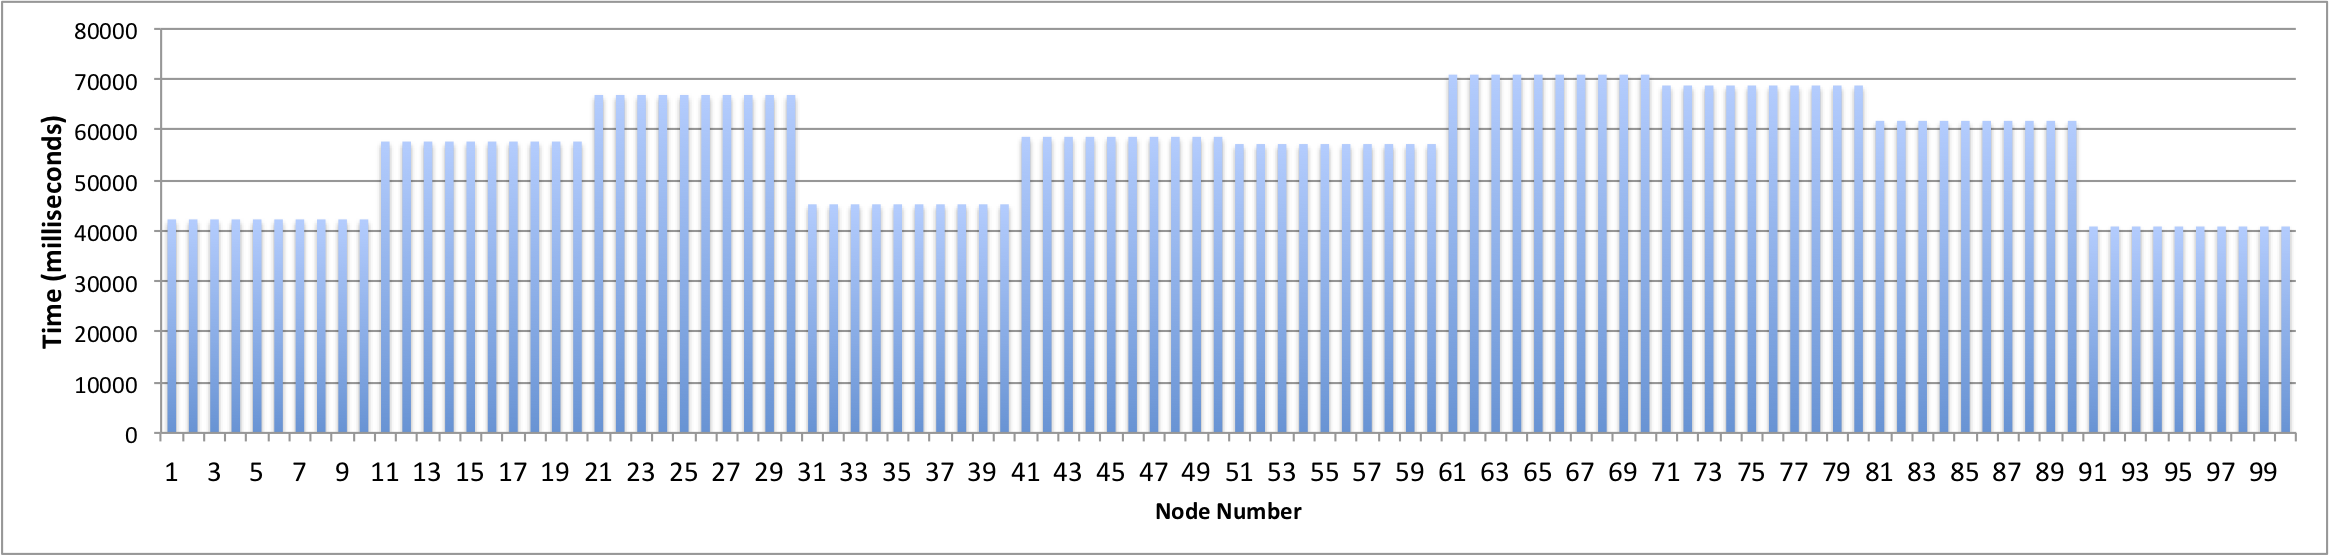
\includegraphics[width=0.9\textwidth]{LoadNodesBal}
\end{center}
\caption{\label{fig:loadNodesBal}Load distribution across cores for 10
  nodes with 10 cores each, when balancing is done within node.}
\end{figure}

\begin{figure}[ht!]
\label{fig:loadNodesBal25}
\begin{center}
\includegraphics[width=0.9\textwidth]{LoadNodesBal25cores}
\end{center}
\caption{\label{fig:loadNodesBal25}Load distribution across
  cores for 10 nodes with 25 cores each, when balancing is done within
  node.}
\end{figure}

\section{Implications} 
%Even though across any consecutive iterations, the correlation is
%small, the across-node . 
This detailed analysis gives us some suggestions for efficient
within-node dynamic load balancing strategies. From my previous work,
we know that a mix of static and dynamic balancing is helpful. A
certain sequence of iterations are assigned to each thread ahead of
time (statically). All the remaining iterations are kept in a dynamic
pool so that idle threads can pick work from this pool. The
persistence from iteration to iteration, combined with the variability
of load across particles, suggests that the static loop iterations
should be assigned in a weighted manner using the timing data from the
previous iteration, i.e., we assign equal amount of predicted work to each
thread, rather than equal number of iterations. Although the
correlation from one iteration to the next is high, the correlation
deteriorates after you go multiple iterations, i.e., the correlation
between 0 and 75 was only 0.53. This suggests that the weighted
assignment of loop iterations to cores needs 
to be adjusted periodically (and this underscores the need for a
sophisticated runtime).

%A weighted factoring would reduce the idle time for each thread. 
%A weighted factoring along with dynamic scheduling could provide 
%further performance gains because of quasi-persistence. 

\bibliographystyle{abbrv}
\bibliography{bibliography}
\end{document}
